\documentclass[11pt,DIV=13,a4paper,parskip=half,abstract=true,ngerman]{scrartcl}
\usepackage[ngerman]{babel}
% \usepackage[margin=2.3cm]{geometry}
\usepackage[T1]{fontenc}
\usepackage[scaled=0.95]{helvet}
\usepackage{microtype}
\usepackage{booktabs}
\usepackage{tabularx}
\usepackage{graphicx}
\usepackage{soul}\sethlcolor{yellow!35}
\usepackage{subcaption}
\captionsetup{font=small,labelfont=bf,labelsep=space}
\captionsetup[sub]{font=small,labelfont=bf}
\usepackage{csquotes}
\usepackage{xurl}
\usepackage[backend=biber,style=authoryear-comp,maxbibnames=4,maxcitenames=2,uniquename=false,urldate=long]{biblatex}
\addbibresource{quellen.bib}
% Jahr nur aus dem Erscheinungsdatum, nie aus dem Abrufdatum (sonst erscheint "2026" bei undatierten Quellen)
\DeclareLabeldate{\field{date}\field{eventdate}\field{origdate}\literal{nodate}}
\DefineBibliographyStrings{ngerman}{nodate={o.\,J\adddot}}
\usepackage{zkopipeline}
% Farben der Wärmeplan-Legende (erzeugt von daten/auswertung.py, gleiche Tabelle wie die Karten)
% erzeugt von daten/auswertung.py -- nicht von Hand ändern
\definecolor{wp-bestand}{HTML}{007256}% Wärmenetzgebiet – Bestand
\definecolor{wp-erw30}{HTML}{489A7D}% Erschließung bis 2030
\definecolor{wp-erw35}{HTML}{9BCFAF}% Erschließung 2030–2035
\definecolor{wp-erw40}{HTML}{C6F2D7}% Erschließung 2035–2040
\definecolor{wp-erw45}{HTML}{D5FEE5}% Erschließung 2040–2045
\definecolor{wp-pruefhoch}{HTML}{9185BE}% Prüfgebiet – hohe Wärmenetzeignung
\definecolor{wp-pruefgeg}{HTML}{F5B4CB}% Prüfgebiet – Wärmenetzeignung gegeben
\definecolor{wp-dezentral}{HTML}{F39300}% Dezentrale Versorgung
\definecolor{wp-ohne}{HTML}{E6E6E6}% Ohne relevanten Wärmebedarf

\usepackage{enumitem}
% Wasserzeichen "Entwurf" auf allen Seiten (hellgrau, hinter dem Text)
\usepackage{draftwatermark}
\DraftwatermarkOptions{text={Entwurf},color=black!7,scale=1.2,angle=45}
% hyperref als letztes Paket: Links, Querverweise und Zitate klickbar, ohne Rahmen/Farbe
\usepackage[hidelinks]{hyperref}
\hypersetup{pdftitle={Marktrollen und Transparenz beim Fernwärmeausbau in Berlin},pdfauthor={Jan Suchanek},
  pdfsubject={Eine Analyse offener Verbrauchs- und Planungsdaten},pdflang={de-DE}}
% \autoref macht "Abb. 4" als Ganzes klickbar, nicht nur die Zahl
\addto\extrasngerman{%
    \def\figureautorefname{Abb.}\def\tableautorefname{Tab.}%
    \def\subfigureautorefname{Abb.}
    \def\sectionautorefname{Abschnitt}}
\setlist{itemsep=2pt,topsep=4pt}

% Beschriftungen mit KOMA-Mitteln: "Abb. 1" fett, Text klein, kein Doppelpunkt
\setkomafont{caption}{\small}
\setkomafont{captionlabel}{\bfseries}
\renewcommand*{\captionformat}{\ }
\renewcaptionname{ngerman}{\figurename}{Abb.}
\renewcaptionname{ngerman}{\tablename}{Tab.}
\renewcaptionname{ngerman}{\abstractname}{Kernaussagen}
\renewcommand{\familydefault}{\sfdefault}
\sisetup{output-decimal-marker={,},group-separator={.},group-minimum-digits=4,mode=text}

% Markierung für Textstellen, die noch zu prüfen oder zu schreiben sind
\newcommand\offen[1]{{\color{zkolight}\textbf{[#1]}}}

% ---------------------------------------------------------------------
% Daten: alle Zahlen im Text stammen aus diesen Dateien (daten/auswertung.py)
% ---------------------------------------------------------------------
\DTLloaddb{kz}{daten/ergebnis/kennzahlen.csv}
\DTLloaddb{gebiete}{daten/ergebnis/gebiete.csv}
\DTLloaddb{stuetz}{daten/ergebnis/stuetzjahre.csv}
\DTLloaddb{betreiber}{daten/ergebnis/betreiber.csv}
\DTLloaddb{kzh}{daten/ergebnis/kennzahlen_hiq.csv}
\DTLloaddb{gebhiq}{daten/ergebnis/gebiete_hiq.csv}
\DTLloaddb{akteure}{daten/ergebnis/akteure_hiq.csv}

% \kzget{schluessel}{\cs}: Kennzahl in Makro holen
\newcommand\kzget[2]{\DTLgetvalueforkey{#2}{wert}{kz}{schluessel}{#1}}
% \kz[stellen]{schluessel}: Kennzahl gerundet ausgeben
\newcommand\kz[2][1]{\kzget{#2}{\kzwert}\zkonum[#1]{\kzwert}}
% dasselbe für die Fallstudie HIQ
\newcommand\kzhget[2]{\DTLgetvalueforkey{#2}{wert}{kzh}{schluessel}{#1}}
\newcommand\kzh[2][0]{\kzhget{#2}{\kzwert}\zkonum[#1]{\kzwert}}

% häufig gebrauchte Werte
\kzget{gas-bez-2023}{\gasbez}  \kzget{fw-bez-2023}{\fwbez}
\kzget{gas-bez-2021}{\gasbezalt} \kzget{fw-bez-2021}{\fwbezalt}
\kzget{gas-block-2023}{\gasblock} \kzget{fw-block-2023}{\fwblock}
\kzget{gas-netz-2045}{\gasnetz} \kzget{gas-bew-allein}{\gasbew}
\kzget{gas-gesperrt-2021}{\gesperrtalt} \kzget{gas-gesperrt-2023}{\gesperrt}
\kzget{gesperrt-netz}{\gesperrtnetz} \kzget{gesperrt-bestand}{\gesperrtbestand}
\kzget{gas-pruef}{\gaspruef}

\title{Marktrollen und Transparenz beim Fernwärmeausbau in Berlin}
\subtitle{Eine Analyse offener Verbrauchs- und Planungsdaten}
\author{Jan Suchanek}
\date{Kurzanalyse, November 2026 \textbullet\ Entwurf}

\begin{document}

\maketitle

\begin{abstract}
    % quotation-Umgebung: Einzug aus, Absatzabstand wie im übrigen Text
    \setlength{\parindent}{0pt}\setlength{\parskip}{0.5\baselineskip}
    Berlin will bis 2045 klimaneutral sein; der im Juni 2026 beschlossene Wärmeplan legt fest, welche Gebiete künftig über Wärmenetze versorgt werden.
    Für die Gaskunden dort wird ein Vertrag auf einem Wettbewerbsmarkt durch einen Vertrag mit einem Monopolanbieter ersetzt.
    Diese Kurzanalyse verschneidet die offenen Verbrauchsdaten des Umweltatlas auf Blockebene mit den Wärmeversorgungsgebieten des Wärmeplans und beziffert so Marktvolumen und Marktstruktur der künftigen Fernwärmeversorgung.

    Rund \zkonum{\gasnetz}~TWh Gas -- das sind \zkoshare{\gasnetz}{\gasblock} des sichtbaren Verbrauchs -- liegen in Gebieten, die bis 2045 Wärmenetzen zugeordnet sind, \zkonum{\gasbew}~TWh davon in Gebieten, für die allein die landeseigene BEW vorgesehen ist.
    Zugleich fehlen auf Blockebene \zkoshare{\gasbez-\gasblock}{\gasbez} des Gas- und \zkoshare{\fwbez-\fwblock}{\fwbez} des Fernwärmeverbrauchs; gesperrte Werte häufen sich dort, wo Großabnehmer mit dem Monopolanbieter verhandeln.
    Das Land ist Eigentümer der BEW, Planer der Gebiete, gebündelter Abnehmer und Sitz der Aufsicht.
    Am Zukunftsort Health Innovation Quarter zeigt sich, wie unterschiedlich die Verhandlungspositionen der Abnehmer sind.

    Daraus folgen Empfehlungen zu Datentransparenz, Preistransparenz für Großkunden und zur Trennung der Rollen des Landes.
\end{abstract}
    



\tableofcontents

% =====================================================================
\section{Ausgangslage}
% =====================================================================

Berlin hat im Juni 2026 seinen Wärmeplan beschlossen \parencite{senat2026waermeplan}.
Er ordnet jedem Teilblock der Stadt ein Wärmeversorgungsgebiet zu und gibt für Wärmenetzgebiete an, bis zu welchem Stützjahr (2030 bis 2045) sie erschlossen werden sollen und welcher Betreiber vorgesehen ist.
Seit 2024 gehört der größte Betreiber, die BEW Berliner Energie und Wärme, wieder dem Land \parencite{senat2024bew}.

Mit dem Ziel der Klimaneutralität bis 2045 endet die Gasheizung im Gebäudebestand \parencite{herpich2023}.
Wo der Wärmeplan Wärmenetze vorsieht, wird ein Gasvertrag auf einem Wettbewerbsmarkt durch einen Fernwärmevertrag mit einem Monopolanbieter ersetzt.
Das ist ein erheblicher Markteingriff: Er betrifft einen großen Teil des heutigen Gasabsatzes, und dieses Volumen ist zugleich die Basis, über die der Umbau der Netze refinanziert werden soll.

Auf diesem künftigen Markt hat das Land mehrere Rollen zugleich.
Es ist Eigentümer des größten Anbieters, legt die Versorgungsgebiete fest, kauft selbst in großem Umfang Fernwärme ein und ist Sitz der zuständigen Aufsicht.
Gleichzeitig ist der Markt öffentlich nur eingeschränkt einsehbar: Verbräuche großer Abnehmer werden aus Datenschutzgründen nicht ausgewiesen, Netzkarten nicht veröffentlicht.

Diese Kurzanalyse fragt deshalb, welches Absatzvolumen der Wärmeplan welchen Betreibern zuweist, wie gut dieser Markt öffentlich einsehbar ist und welche Rollen das Land darin einnimmt.
Dazu verbindet sie zwei offene Datenquellen, die bislang getrennt betrachtet werden: die Verbrauchsdaten des Umweltatlas auf Blockebene und die Wärmeversorgungsgebiete des Wärmeplans.
Gemeinsam geben sie Aufschluss über Marktvolumen und Marktstruktur der künftigen Fernwärmeversorgung.
\autoref{sec:stand} ordnet die Fragestellung in die Debatte ein, die Abschnitte~\ref{sec:volumen} bis~\ref{sec:aufsicht} enthalten die Befunde, \autoref{sec:hiq} vertieft sie am Beispiel eines Zukunftsorts.

% =====================================================================
\section{Stand der Diskussion}\label{sec:stand}
% =====================================================================

Fernwärmenetze sind natürliche Monopole; anders als bei Strom und Gas gibt es weder eine Trennung von Netz und Vertrieb noch eine Regulierung der Netzentgelte.
Die Monopolkommission empfiehlt deshalb kurzfristig eine Transparenzplattform, überarbeitete Preisgleitklauseln und eine vereinfachte Price-Cap-Regulierung, langfristig eine gesetzliche Zugangsregulierung für Dritte \parencite{monopolkommission2024,monopolkommission2025}.
Das Bundeskartellamt hat in vier von neun untersuchten Netzen den Verdacht rechtswidriger Preisanpassungsklauseln erhärtet \parencite{bkarta2023,bkarta2025}, der Verbraucherzentrale Bundesverband fordert eine bundeseinheitliche Preisaufsicht \parencite{vzbv2024}.
Die Eckpunkte des Wärmenetzpakets vom August 2026 sehen eine Transparenzplattform und eine nachträgliche Preisaufsicht durch eine Bundesbehörde vor, nicht aber Preisobergrenzen oder Netzzugang \parencite{bmwe2026waermenetzpaket}.

Die Branchenverbände halten dagegen, steigende Preise seien Folge des Investitionsbedarfs, nicht fehlenden Wettbewerbs \parencite{bdew2024monopolkommission,zfk2025monopolkommission}.
Dieser Bedarf ist groß: Für die städtische Fernwärme werden bis 2045 rund 74,4~Mrd.\,Euro veranschlagt \parencite{prognos2024}, der Umbau bestehender Großstadtnetze gilt unter heutigen Bedingungen als kaum refinanzierbar \parencite{ariadne2023}.
Für Strom-, Gas- und Wärmenetze zusammen beziffern \textcite{inan2025} den Investitionsbedarf der Versorger bis 2045 auf rund 627~Mrd.\,Euro, davon 63~Mrd.\,Euro zusätzliches Eigenkapital; Bund und Länder haben dazu im Oktober 2026 Eckpunkte vorgelegt \parencite{bmf2026netze}.
Die dena diskutiert Preisregulierung deshalb vor allem von der Finanzierungsseite \parencite{dena2025}.
Wer die Investitionen über Preise trägt, ist die Kehrseite der Regulierungsfrage; zu den Verteilungswirkungen auf Gebäudeseite vgl.\ \textcite{henze2026}.

Für Berlin zeigt das DIW, dass Fernwärme-, Strom- und Gasnetze für den Ausstieg aus dem Erdgas gemeinsam geplant werden müssen \parencite{herpich2023}; der Wärmeplan legt diese Planung nun räumlich fest.
International gilt der Netzzugang für Dritte in lokalen Netzen als wenig wirksam, bei ausgeprägtem natürlichem Monopol wird eine Preisregulierung im Voraus empfohlen \parencite{soederholm2011,buerger2019}.
Die Niederlande verbinden seit 2025 einen verpflichtenden öffentlichen Mehrheitsanteil an Wärmeunternehmen mit einer kostenbasierten Tarifregulierung \parencite{wcw2025,vng2025wcw}.
Berlin hat das öffentliche Eigentum, aber keine unabhängige Regulierung.

Die genannten Beiträge argumentieren überwiegend auf Bundesebene und ohne räumlichen Bezug.
Diese Kurzanalyse ergänzt sie um drei Punkte: eine räumliche Quantifizierung des Absatzvolumens, das ein Wärmeplan einzelnen Betreibern zuweist; die Datenlage selbst als Befund; und die Doppelrolle eines Landes als Eigentümer, Planer, Abnehmer und Sitz der Aufsicht.

% =====================================================================
\section{Gasverbrauch in künftigen Wärmenetzgebieten}\label{sec:volumen}
% =====================================================================

\begin{figure}[ht]
\centering
\zkobars[unit=TWh,width=6.5,color=farbe]{gebiete}{gas-twh}
\caption{Gasverbrauch 2023 (sichtbare Blockwerte) nach
Wärmeversorgungsgebiet laut Wärmeplan 2045.\\ Quelle: Umweltatlas, Wärmeplan Berlin;
eigene Verschneidung.}\label{fig:gebiete}
\end{figure}

Von den \zkonum{\gasblock}~TWh Gas, die auf Blockebene sichtbar sind, liegen \zkonum{\gasnetz}~TWh in Gebieten, die bis 2045 an ein Wärmenetz angeschlossen werden sollen (\autoref{fig:gebiete}).
Der größte Teil, \kz{gas-bestand}~TWh, liegt bereits heute in Fernwärmegebieten; hier geht es um Nachverdichtung.
Weitere \zkonum{\gaspruef}~TWh liegen in Prüfgebieten, die überwiegend als wärmenetzgeeignet gelten, nur \kz{gas-dezentral}~TWh in Gebieten für dezentrale Versorgung wie Wärmepumpen.

\begin{figure}[ht]
    \centering
    \DTLmaxforcolumn{stuetz}{gas-twh}{\stmax}%
    \subcaptionbox{kumuliert nach Stützjahr\label{fig:stuetz}}{%
        % gestapelte Balken: Segmente in den Kartenfarben, Summe am Balkenende
        \begin{tikzpicture}[font=\sffamily\footnotesize]
        \DTLforeach*{stuetz}{\stj=jahr,\sta=bestand,\stb=erw30,\stc=erw35,\std=erw40,\ste=erw45,\stt=gas-twh}{%
          \edef\sty{\fpeval{-0.6*\DTLcurrentindex}}%
          \gdef\stx{0}%
          \foreach \v/\f in {\sta/wp-bestand,\stb/wp-erw30,\stc/wp-erw35,\std/wp-erw40,\ste/wp-erw45}{%
            \zkotest{\v > 0}{%
              \edef\stw{\fpeval{3.4*\v/\stmax}}%
              \filldraw[fill=\f,draw=black!35,line width=0.3pt] (\stx cm,\sty) rectangle ++(\stw cm,0.42);
              \xdef\stx{\fpeval{\stx+\stw}}}{}}
          \node[left] at (0,\sty+0.21) {\stj};
          \node[right] at (\stx cm,\sty+0.21) {\zkonum{\stt}\,TWh};
        }
        \end{tikzpicture}}%
    \hspace{3em}%
    \subcaptionbox{nach vorgesehenem Betreiber (2045)\label{fig:betreiber}}{%
        \zkobars[unit=TWh,width=2.6,color=farbe]{betreiber}{gas-twh}}
    \caption{Gas 2023 in Wärmenetzgebieten.}\label{fig:netzgas}
\end{figure}

Der Großteil dieses Volumens entfällt auf ein Unternehmen (\autoref{fig:betreiber}): In Gebieten, für die allein die BEW vorgesehen ist, wurden 2023 \zkonum{\gasbew}~TWh Gas verbraucht, rechnerisch \zkoshare{\gasbew}{\fwbez} des heutigen Berliner Fernwärmeverbrauchs von \zkonum{\fwbez}~TWh.
Das ist eine Obergrenze vor Sanierung, die der Plan mit 1{,}7\,\% pro Jahr ansetzt \parencite{senmvku2026kernaussagen}.
Die BEW sieht im Wärmeplan entsprechend eine Grundlage für ihren weiteren Ausbau und für höhere Anschlussgrade in bestehenden Netzen \parencite{bew2026gb}.
Über dieses Volumen soll der Umbau refinanziert werden; 2025 investierte die BEW rund 422~Mio.\,Euro \parencite{bew2026gb}.
Wie die Preise zustande kommen, wird damit zur zentralen Frage.

% =====================================================================
\section{Datenlage und Transparenz}\label{sec:daten}
% =====================================================================

\begin{figure}[ht]
    \centering
    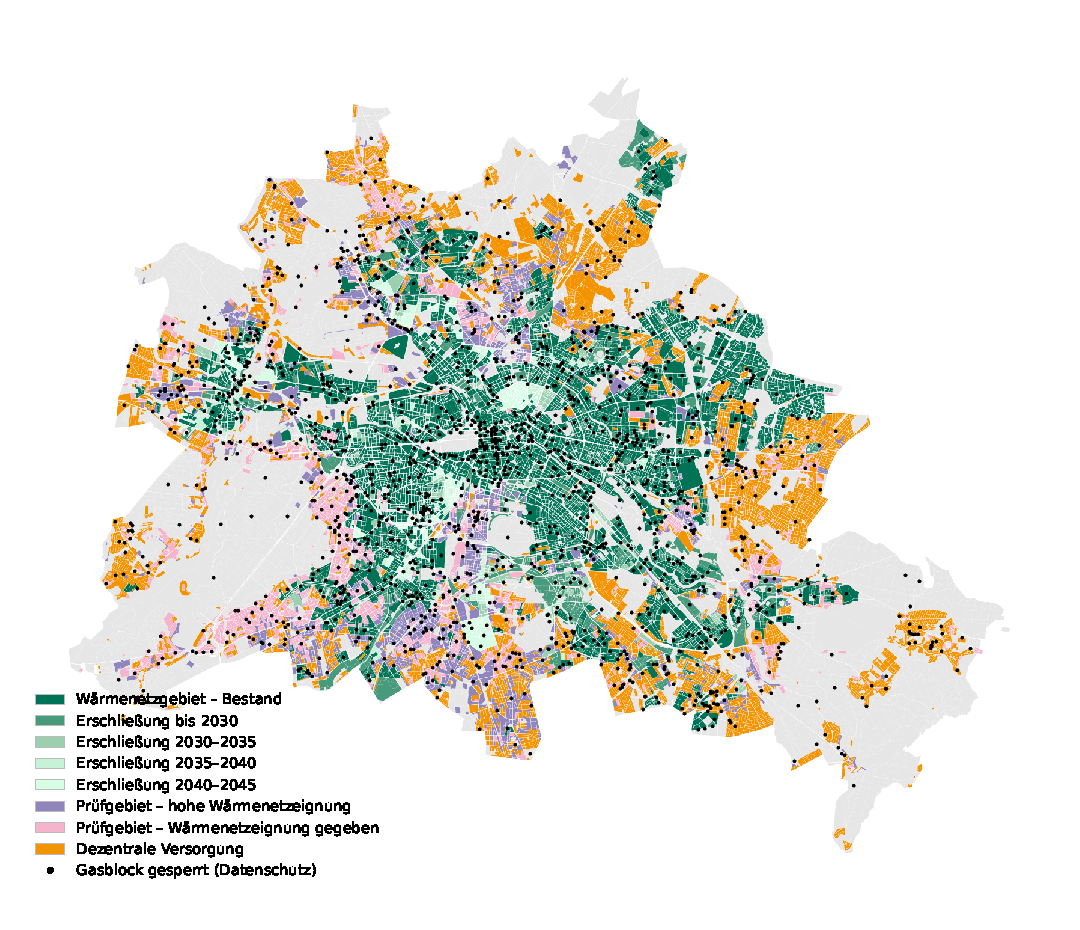
\includegraphics[width=\linewidth]{abb/karte.pdf}
    \caption{Wärmeversorgungsgebiete 2045 (Farben der offiziellen
    Wärmeplan-Legende) und gesperrte Gasblöcke (Punkte). Quelle: Wärmeplan Berlin, Umweltatlas.}\label{fig:karte}
\end{figure}

Der Umweltatlas sperrt Blockwerte, wenn zu wenige Abnehmer Rückschlüsse auf Einzelne erlauben; gesperrte Blöcke enthalten daher typischerweise einen oder wenige große Verbraucher.
Die Summe der sichtbaren Blockwerte bleibt beim Gas um \zkoshare{\gasbez-\gasblock}{\gasbez}, bei der Fernwärme um \zkoshare{\fwbez-\fwblock}{\fwbez} hinter den Bezirkssummen zurück.
Die Zahl gesperrter Gasblöcke stieg von \zkonum[0]{\gesperrtalt} (2021) auf \zkonum[0]{\gesperrt} (2023), sprunghaft zwischen 2021 und 2022; ob mehr Großabnehmer oder eine geänderte Veröffentlichungspraxis die Ursache sind, lässt sich aus den Daten nicht bestimmen.
\zkoshare{\gesperrtnetz}{\gesperrt} der gesperrten Blöcke liegen in künftigen Wärmenetzgebieten, \zkonum[0]{\gesperrtbestand} allein in heutigen Fernwärmegebieten (\autoref{fig:karte}).
Hinzu kommen zwei weitere Lücken: Der Fernwärme-Datensatz weist nicht aus, ob ein fehlender Wert gesperrt ist oder kein Anschluss besteht, und die Netzkarten des Wärmeplans werden aus Gründen des Infrastrukturschutzes nicht veröffentlicht \parencite{senmvku2026karten}.

Ökonomisch ist das der kritische Punkt.
Ein großer Abnehmer in einem Fernwärmegebiet steht einem Monopolanbieter gegenüber und kann kaum ausweichen -- ein \emph{bilaterales Monopol}, in dem der Preis verhandelt wird, für Außenstehende unsichtbar.
Wie stark ein Abnehmer verhandeln kann, hängt von seiner Ausweichmöglichkeit ab (\autoref{tab:typen}); im Health Innovation Quarter (\autoref{sec:hiq}) finden sich alle diese Typen.

\begin{table}[ht]
    \small\centering
    \begin{tabularx}{\linewidth}{@{}>{\raggedright}p{2.8cm}>{\raggedright}p{3.4cm}>{\raggedright\arraybackslash}X>{\raggedright\arraybackslash}p{3.0cm}@{}}
        \toprule
        Abnehmer & Beispiel im HIQ & Ausweichmöglichkeit & Verhandlungsposition \\
        \midrule
        Industrie & Standort Müllerstraße & eigene Erzeugung, Prozesswärme & vergleichsweise stark \\
        Landeseinrichtungen mit eigener Anlage & Campus Virchow-Klinikum & eigene KWK-Anlage im Contracting & begrenzt, an Vertragslaufzeit gebunden \\
        Bund & BND, Ministerien, Bundeswehrkrankenhaus & Bündelung (BImA), eigene Erzeugung möglich & mittel, politisches Gewicht \\
        Landeseinrichtungen im Rahmenvertrag & Campus Charité Mitte & keine & keine im üblichen Sinn: Käufer und Eigentümer sind dasselbe Land \\
        Kleinabnehmer & Wohngebäude & keine & Standardtarif \\
        \bottomrule
    \end{tabularx}
    
    \caption{Verhandlungsmacht gegenüber dem Fernwärmeversorger. Zuordnung der
    Beispiele nach Lage und öffentlich zugänglichen Angaben; die Teilnahme der Charité am Rahmenvertrag ist öffentlich nicht dokumentiert.}\label{tab:typen}
\end{table}

% =====================================================================
\section{Zuständigkeiten und Aufsicht}\label{sec:aufsicht}
% =====================================================================

Die Preismissbrauchsaufsicht über einen Versorger, der nur in einem Land tätig ist, liegt bei der Landeskartellbehörde (§\,48 Abs.\,2 GWB).
In Berlin gehört sie, wie die Regulierungsbehörde für Fernwärme, zur Senatsverwaltung für Wirtschaft, Energie und Betriebe.
Kostenkalkulationen der Wärmenetzbetreiber kann der Senat nach eigener Auskunft nur im Rahmen der Missbrauchsaufsicht erheben; für Preise verweist er auf eine freiwillige Plattform der Branchenverbände \parencite{agh2026s1926754}.

Die BEW gehört dem Land mittelbar zu 100\,\% \parencite{senfin2025unternehmen}.
Der Senat beschließt für sie jährlich finanz- und fachpolitische Ziele, die in Zielvereinbarungen mit der Geschäftsführung münden \parencite{senat2024beteiligungsgrundsaetze,senfin2025beteiligung}.
Den Aufsichtsratsvorsitz führt laut Geschäftsbericht 2025 die Senatorin für Wirtschaft, Energie und Betriebe, deren Verwaltung zugleich die Aufsicht führt \parencite{bew2026gb}.
Die Ziele des Eigentümers und das Interesse der Kunden an niedrigen Preisen werden damit innerhalb derselben Landesregierung abgewogen, ohne dass dies von außen nachvollziehbar ist.
Die Finanzbeziehungen sind erheblich: 2024 führte das Land der BEW 495~Mio.\,Euro Eigenkapital zu, der Klimapakt von 2025 sieht weitere 550~Mio.\,Euro vor, und 2025 zahlte die BEW 56~Mio.\,Euro an die Landesholding aus.
Der Durchschnittserlös lag 2025 bei rund \zkonum{100*1145.0/8576}~ct/kWh (Umsatz 1.145~Mio.\,Euro, Absatz 8.576~GWh); durch einen neuen Tarif stiegen die Leistungserlöse um 50,6~Mio.\,Euro \parencite{bew2026gb}.

Zugleich ist das Land der größte gebündelte Abnehmer.
Die Energiewirtschaftsstelle kauft Fernwärme zentral für Verwaltung, Hochschulen und Krankenhäuser ein, rund 850~GWh im Jahr an etwa 1.700 Abnahmestellen \parencite{ews}, auf Grundlage einer Rahmenvereinbarung mit dem Versorger \parencite{agh2023s1917214} -- seit 2024 also mit dem eigenen Unternehmen.
Der Preis dieses Vertrags ist eine Verrechnung zwischen öffentlichen Haushalten; ob er über oder unter dem liegt, was vergleichbare private Abnehmer zahlen, lässt sich von außen nicht prüfen.
Ob die Charité an dem Vertrag teilnimmt, geht aus den öffentlichen Angaben nicht hervor.

% =====================================================================
\section{Empfehlungen}\label{sec:empfehlungen}
% =====================================================================

\begin{enumerate}[leftmargin=16pt]
    \item \textbf{Messbarkeit der Datenlücke.}
    Der Umweltatlas sollte für Fernwärme wie für Gas ausweisen, ob ein fehlender Wert gesperrt ist oder kein Anschluss besteht.
    Gesperrte Werte sollten zudem aggregiert je Wärmeversorgungsgebiet veröffentlicht werden: Der Schutz einzelner Abnehmer bleibt gewahrt, die Lücke wird aber bezifferbar.
    Ohne diese Angaben lässt sich nicht prüfen, wie viel Absatz der Wärmeplan tatsächlich umlenkt.

    \item \textbf{Preistransparenz auch für Großkunden.}
    Die geplante Bundesplattform sollte neben Standardtarifen eine anonymisierte Verteilung der Preise aus Sonderkundenverträgen je Netzgebiet enthalten, etwa in Quartilen.
    Großabnehmer verhandeln im bilateralen Monopol individuell; ihre Konditionen bestimmen mit, wie die Kosten des Umbaus zwischen den Kundengruppen verteilt werden.
    Eine Verteilung genügt, einzelne Verträge müssen nicht offengelegt werden.

    \item \textbf{Trennung der Rollen.}
    Für Wärmeversorger im Eigentum eines Landes sollte die künftige Preisaufsicht bei der Bundesbehörde des Wärmenetzpakets liegen, nicht in der Landesverwaltung, die zugleich die Eigentümerziele setzt.
    Das entspricht der Logik der Netzregulierung bei Strom und Gas, wo die Aufsicht unabhängig vom Eigentum der Netze ist.
    Bis dahin sollten Aufsichtsratsvorsitz und Kartellaufsicht zumindest nicht in derselben Senatsverwaltung liegen.

    \item \textbf{Offenlegung von Rahmenvertrag und Eigentümerzielen.}
    Preis, Menge und Anpassungsklauseln der Rahmenvereinbarung zwischen Land und BEW betreffen öffentliche Mittel auf beiden Seiten und wären ein Maßstab für alle übrigen Abnehmer.
    Gleiches gilt für die finanzpolitischen Ziele, die der Senat der BEW als Eigentümer vorgibt, etwa Ausschüttungserwartungen.
    Beides ließe sich im Beteiligungsbericht veröffentlichen, ohne Geschäftsgeheimnisse Dritter zu berühren.

    \item \textbf{Ausnahme öffentlicher Abnehmer von der Sperrregel.}
    Die Sperrregel schützt Einzelpersonen und Unternehmen; für öffentliche Einrichtungen, deren Energiekosten aus öffentlichen Mitteln bezahlt werden, gibt es keinen vergleichbaren Grund.
    Bislang richtet sie sich allein nach der Zahl der Verbrauchsstellen: Im Health Innovation Quarter ist der Gasverbrauch eines Universitätsklinikums gesperrt, der eines Nachrichtendienstes sichtbar (\autoref{sec:hiq}).
    Ausnahmen sollten sich nach der Schutzbedürftigkeit richten, etwa für sicherheitsrelevante Standorte.
\end{enumerate}

Gegen diese Empfehlungen lässt sich der Investitionsbedarf anführen.
Der BDEW unterstützt eine stärkere Preisaufsicht grundsätzlich, warnt aber vor Doppelregulierung; neue Instrumente sollten an die Missbrauchsaufsicht anknüpfen, Preisdeckel ausgeschlossen und Investitionen refinanzierbar bleiben \parencite{bdew2026presse,bdew2026stellungnahme}.
Dieser Einwand ist ernst zu nehmen, spricht aber nicht gegen Transparenz: Gerade wenn Investitionen über Preise refinanziert werden, muss nachvollziehbar sein, wer sie trägt.
Die Empfehlungen betreffen deshalb die Offenlegung von Mengen, Preisen und Zuständigkeiten, nicht deren Höhe; wo Datenschutz oder Infrastrukturschutz entgegenstehen, genügen aggregierte Angaben.

% =====================================================================
\section{Fallstudie: Health Innovation Quarter}\label{sec:hiq}
% =====================================================================

\kzhget{hiq-innerhalb-gas}{\hgas} \kzhget{hiq-innerhalb-fw}{\hfw}
\kzhget{hiq-blockflaeche-ha}{\hha} \kzhget{berlin-blockflaeche-ha}{\bha}
\kzhget{berlin-gas-gwh}{\bgas} \kzhget{hiq-gas-top2}{\htop}
\kzhget{hiq-innerhalb-bloecke}{\hbl} \kzhget{hiq-gesperrt}{\hges}
\kzhget{berlin-bloecke}{\bbl} \kzhget{berlin-gesperrt}{\bges}
\kzhget{hiq-gas-netz}{\hnetz}
\kzhget{hiq-gas-top1}{\hone} \kzhget{hiq-top1-ha}{\honeha} \kzhget{hiq-top2-ha}{\htopha}
\DTLgetvalueforkey{\bndgas}{gas-gwh}{akteure}{id}{bnd}

Berlin weist aktuell elf Orte als \enquote{Zukunftsorte} aus: Standorte, an denen Netzwerke zwischen Wissenschaft und Wirtschaft bestehen oder ausgebaut werden sollen und die das Land als Baustein seiner Wirtschafts- und Innovationspolitik fördert \parencite{zko}.
2026 neu ausgewiesen wurde das Health Innovation Quarter Berlin-Mitte (HIQ), initiiert von Charité und Bayer; es erstreckt sich als Band von rund fünf Kilometern vom Campus Charité Mitte über den Bayer-Standort bis zum Campus Virchow-Klinikum \parencite{zkohiq}.
Der hier verwendete Umriss umfasst zwei Teilflächen mit zusammen \kzh{hiq-ha}~ha, die Geschäftsstelle nennt rund 250~ha.\footnote{Umriss nachgezeichnet nach \textcite{blc2026wirtschaftsatlas}; er ist nicht als Geodatensatz veröffentlicht.}
Vollständig darin liegen \zkonum[0]{\hbl} statistische Blöcke; \autoref{tab:regel} zeigt, dass die Ergebnisse gegenüber der Auswahlregel robust sind.

\begin{figure}[ht]
    \centering
    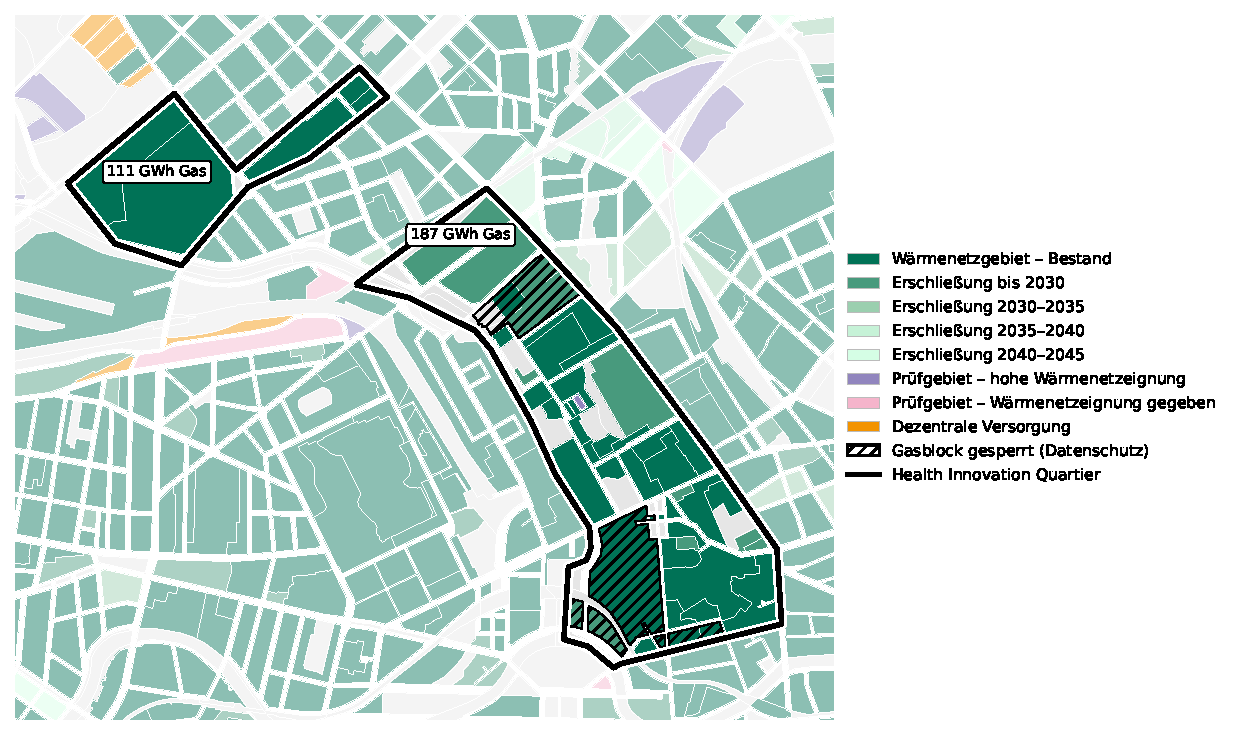
\includegraphics[width=0.95\linewidth]{abb/karte_hiq.pdf}
    \caption{Health Innovation Quarter (schwarzer Umriss):
    Wärmeversorgungsgebiete 2045 (Farben der offiziellen Wärmeplan-Legende), gesperrte Gasblöcke (schraffiert) und die zwei verbrauchsstärksten Blöcke; Umgebung aufgehellt. Quelle: Wärmeplan Berlin, Umweltatlas, eigener Umriss.}\label{fig:hiq}
\end{figure}

Die Blöcke verbrauchten 2023 sichtbar \zkonum[0]{\hgas}~GWh Gas und \zkonum[0]{\hfw}~GWh Fernwärme, dominiert von wenigen Großabnehmern (\autoref{tab:akteure}).
Zwei Blöcke stehen für \zkonum[0]{\htop}~GWh oder \zkoshare{\htop}{\hgas} des sichtbaren Gasverbrauchs: ein Industriestandort an der Müllerstraße (Bayer, \zkonum[0]{\hone}~GWh) und der Campus Virchow-Klinikum.\footnote{Der Umweltatlas nennt keine Verbraucher; die Zuordnung beruht auf der Lage der Blöcke und den Adressen der Akteure.}
An dritter Stelle folgt der Block des Bundesnachrichtendienstes mit \zkonum[0]{\bndgas}~GWh, in einem Gebiet, das bis 2030 an die Fernwärme angeschlossen werden soll.
Je Hektar Blockfläche ist der Gasverbrauch rund \zkonum[0]{(\hgas/\hha)/(\bgas/\bha)}-mal so hoch wie im Berliner Durchschnitt, ohne die beiden Großblöcke noch rund \zkonum[0]{((\hgas-\htop)/(\hha-\htopha))/(\bgas/\bha)}-mal.

Der Campus Virchow-Klinikum wird seit 2017 von einer eigenen Energiezentrale mit Kraft-Wärme-Kälte-Kopplung versorgt, die ein Contractor für 15 Jahre betreibt \parencite{agh2021s1826180,ikz2017charite,dbz2019charite}; das Gas dort ist überwiegend Brennstoff für Strom, Wärme und Kälte.
Mit dem rechnerischen Vertragsende um 2032 steht die Charité vor der Wahl, die Anlage zu erneuern oder sich an die Fernwärme anzuschließen; der Campus liegt vollständig im Bestandsgebiet der BEW.
Ihre Verhandlungsposition hängt davon ab, ob die eigene Option glaubwürdig bleibt.

Zugleich ist das Quartier schlechter einsehbar als die Stadt insgesamt: \zkonum[0]{\hges} der \zkonum[0]{\hbl} Blöcke (\zkoshare{\hges}{\hbl}) sind gesperrt, gegenüber \zkoshare{\bges}{\bbl} in ganz Berlin.
Sie umfassen \kzh{hiq-gesperrt-ha}~ha, darunter nahezu den gesamten Campus Mitte der Charité (\autoref{fig:hiq}), dessen Fernwärmebezug sichtbar ist, sein Gasverbrauch aber nicht -- anders als der des Bundesnachrichtendienstes.
Gesperrt ist auch der Block, in dem Futurium und Bundesforschungsministerium liegen; ob er Fernwärme bezieht, lässt sich mangels Statusfeld nicht erkennen.
Die Sperrung folgt allein der Zahl der Verbrauchsstellen, nicht der Schutzbedürftigkeit eines Standorts.

\begin{table}[ht]
    \small\centering
    \begin{tabular}{@{}llrrl@{}}
        \toprule
        Akteur (Hauptadresse) & Träger & Gas (GWh) & Fernwärme (GWh) & Wärmenetz \\
        \midrule
        \DTLforeach*{akteure}{\aname=name,\atr=traeger,\agas=gas-gwh,\ast=gas-status,\afw=fw-gwh,\awp=wvg-kurz}{%
        \DTLiffirstrow{}{\\}%
        \aname & \atr & \DTLifnullorempty{\agas}{\ast}{\zkonum{\agas}} & \DTLifnullorempty{\afw}{--}{\zkonum{\afw}} & \awp}\\
        \bottomrule
    \end{tabular}
    \caption{Akteure im Health Innovation Quarter und Verbrauch 2023 ihres Blocks. Zuordnung über die Hauptadresse (Adressdienst des Geoportals Berlin); ein Block kann mehrere Nutzer enthalten, große Standorte erstrecken sich über mehrere Blöcke. Akteure nach \textcite{zkohiq}, ergänzt um Bundeseinrichtungen.}\label{tab:akteure}
\end{table}

\zkoshare{\hnetz}{\hgas} des sichtbaren Gasverbrauchs liegen in Wärmenetzgebieten, für die ausschließlich die BEW vorgesehen ist.
Im Quartier treffen damit alle Abnehmertypen aus \autoref{tab:typen} auf denselben, landeseigenen Anbieter -- in einem Quartier, das das Land selbst als Zukunftsort fördert.
Ob es seine Wärme künftig bezahlbar und klimaneutral bezieht, entscheidet sich an Verträgen, die öffentlich nicht einsehbar sind; hier wären die Empfehlungen~2 und~4 besonders aufschlussreich.

{\small
\begin{center}
    \begin{tabular}{@{}lrrr@{}}
    \toprule
    Auswahlregel & Blöcke & Gas (GWh) & Fernwärme (GWh) \\
    \midrule
    vollständig im Umriss (Hauptregel) & \kzh{hiq-innerhalb-bloecke} & \kzh{hiq-innerhalb-gas} & \kzh{hiq-innerhalb-fw} \\
    mehr als 50\,\% der Blockfläche & \kzh{hiq-mehrheit-bloecke} & \kzh{hiq-mehrheit-gas} & \kzh{hiq-mehrheit-fw} \\
    schneidet den Umriss & \kzh{hiq-schneidet-bloecke} & \kzh{hiq-schneidet-gas} & \kzh{hiq-schneidet-fw} \\
    \bottomrule
\end{tabular}

\captionof{table}{Empfindlichkeit gegenüber der Auswahlregel. Der Gasverbrauch ist robust;
bei der Fernwärme kommen Randblöcke hinzu.}\label{tab:regel}
\end{center}}

% =====================================================================
\addsec{Methode und Grenzen}
% =====================================================================

{\small
Gasverbrauch 2023 je Block \parencite{geoportal2026gas} wurde flächenanteilig auf die Teilblöcke des Wärmeplans 2026 \parencite{geoportal2026wp} verteilt; Fernwärme- und Bezirksdaten aus \textcite{geoportal2026fw}. 
Gasverbrauch ist nicht gleich Wärmebedarf (Kochgas, Prozesswärme, Wirkungsgrade); die Werte sind nicht witterungsbereinigt. 
Die Differenz zwischen Block- und Bezirkssummen kann neben gesperrten Werten auch nicht zuordenbare Verbräuche enthalten. 
Die Akteure im Health Innovation Quarter wurden über den Adressdienst des Geoportals Berlin ihren Blöcken zugeordnet. 
\hl{Alle Verbrauchs-, Flächen- und Gebietszahlen in diesem Text werden beim Kompilieren aus den Daten berechnet.}
\hl{Ein Skript ruft dazu die offenen Geodaten des Umweltatlas und des Wärmeplans über die WFS-Dienste des Geoportals Berlin ab, verschneidet sie und schreibt die Ergebnisse in Tabellen, aus denen die Grafiken und Zahlen im Text entstehen.}
\hl{Angaben aus anderen Quellen sind als solche zitiert.}
Die zugrunde liegende Pipeline ist dokumentiert unter \url{https://github.com/penta-jan/zko-pipeline};
Code und Daten dieser Analyse: \url{https://github.com/penta-jan/Fernwaerme-Berlin-Kurzanalyse}.\par
}

\printbibliography[heading=bibintoc,title={Quellen}]

\end{document}
